\subsection{RF-based strategy selection} 
\label{sec:rf_selector}

The efficiency of the B-VND intensification phase depends not only on the selected neighborhood operator but also on the exploration strategy used within that neighborhood. In the original GVNS framework, local search is performed using a First Improvement (FI) strategy, where candidate moves are evaluated sequentially and the search terminates as soon as an improving move is identified. This approach is computationally efficient and allows rapid progression through large neighborhoods.

An alternative strategy is Best Improvement (BI), which evaluates all admissible moves before selecting the most profitable one. Although BI generally provides stronger intensification, it incurs substantially higher computational costs, particularly for expensive neighborhoods such as cross-exchange and 2-opt* on large synchronized instances.

Preliminary analyses conducted on GVNS+ indicated that neither strategy consistently dominates the other. FI is generally advantageous during early search phases, where improving moves are abundant and rapid progress is desirable. Conversely, BI becomes more beneficial near local optima, where improvements are rarer and a more exhaustive exploration can uncover higher-quality moves. The effectiveness of each strategy therefore depends on the current optimization context, including the search stage, neighborhood type, stagnation level, and solution structure.

Rather than selecting a single exploration strategy for the entire optimization process, the problem is reformulated as a contextual decision task in which the algorithm dynamically chooses between FI and BI according to the current search state.

%% ======== Two-head RF selector architecture =========
\subsubsection{Two-head Random Forest strategy selector}
The proposed selector is based on a two-head Random Forest (RF) architecture. Both heads operate on the unified search-state representation introduced in Section~\ref{sec:learning_infra}, which combines instance descriptors, dynamic search indicators, solution characteristics, and neighborhood-context information.

The first head is formulated as a binary classification task estimating the probability that a given strategy will produce an improving move:

\begin{equation}
P(\text{success}\mid s,\text{strategy}),
\label{eq:rf_prob}
\end{equation}

where a successful move corresponds to a strictly positive improvement of the augmented objective function.

The second head is formulated as a regression task estimating the expected normalized improvement:

\begin{equation}
\Delta_{\text{rel}}
=
\frac{F_{\text{before}}-F_{\text{after}}}
{1+F_{\text{before}}},
\label{eq:rf_gain}
\end{equation}

where $F$ denotes the augmented objective function.

This decomposition enables the model to distinguish between the reliability of a strategy and the magnitude of the expected improvement. A strategy may frequently produce small gains or occasionally generate larger improvements, and modeling these aspects separately improves both interpretability and robustness.

%% ======== Training procedure =========
\subsubsection{Training procedure}
Training data are generated using the learning infrastructure presented previously. For each training instance, GVNS+ is executed twice: once using FI exclusively and once using BI exclusively. During these executions, all local-search decisions are recorded together with the corresponding search-state descriptors and optimization outcomes.

Each recorded observation is transformed into a supervised-learning sample by augmenting the search-state representation with an indicator specifying the evaluated strategy. The resulting dataset is then used to train the classifier and regressor independently.

The classifier learns to predict the probability of obtaining an improving move, whereas the regressor estimates the expected normalized improvement. Both models use identical Random Forest configurations, whose hyperparameters are reported in Appendix~B.

%% ======== Online decision mechanism =========
\subsubsection{Online decision mechanism}
During optimization, the selector evaluates the current search state under two hypothetical scenarios corresponding to FI and BI.

Given a feature vector $\mathbf{x}$ describing the current optimization context, two augmented representations are generated:

\begin{equation}
\mathbf{x}_{FI}
=
[\mathbf{x},0],
\label{eq:xfi}
\end{equation}

\begin{equation}
\mathbf{x}_{BI}
=
[\mathbf{x},1].
\label{eq:xbi}
\end{equation}

The classifier and regressor evaluate both representations and produce four predictions:

\[
P_{FI},\quad G_{FI},\quad
P_{BI},\quad G_{BI},
\]

where $P$ denotes the predicted success probability and $G$ the expected normalized gain.

The final score associated with each strategy is computed as

\begin{equation}
S_{FI}
=
P_{FI}\max(G_{FI},0),
\label{eq:sfi}
\end{equation}

\begin{equation}
S_{BI}
=
P_{BI}\max(G_{BI},0).
\label{eq:sbi}
\end{equation}

Negative predicted gains are clipped to zero in order to avoid rewarding deteriorating moves. The strategy associated with the largest score is selected for neighborhood exploration.

This multiplicative scoring rule naturally balances reliability and expected improvement magnitude. Strategies that appear promising but unreliable receive lower scores, while highly reliable strategies producing only negligible gains are also penalized.

Figure~\ref{fig:rf_internal_layout} and Figure~\ref{fig:rf_inference} summarize the complete online inference procedure.

\begin{figure}[ht]
\centering

\includegraphics[width=\linewidth]
{../figures/rf_internal_layout.pdf}

\caption{RF internal layout}
\label{fig:rf_internal_layout}
\end{figure}

\begin{figure}[ht]
\centering
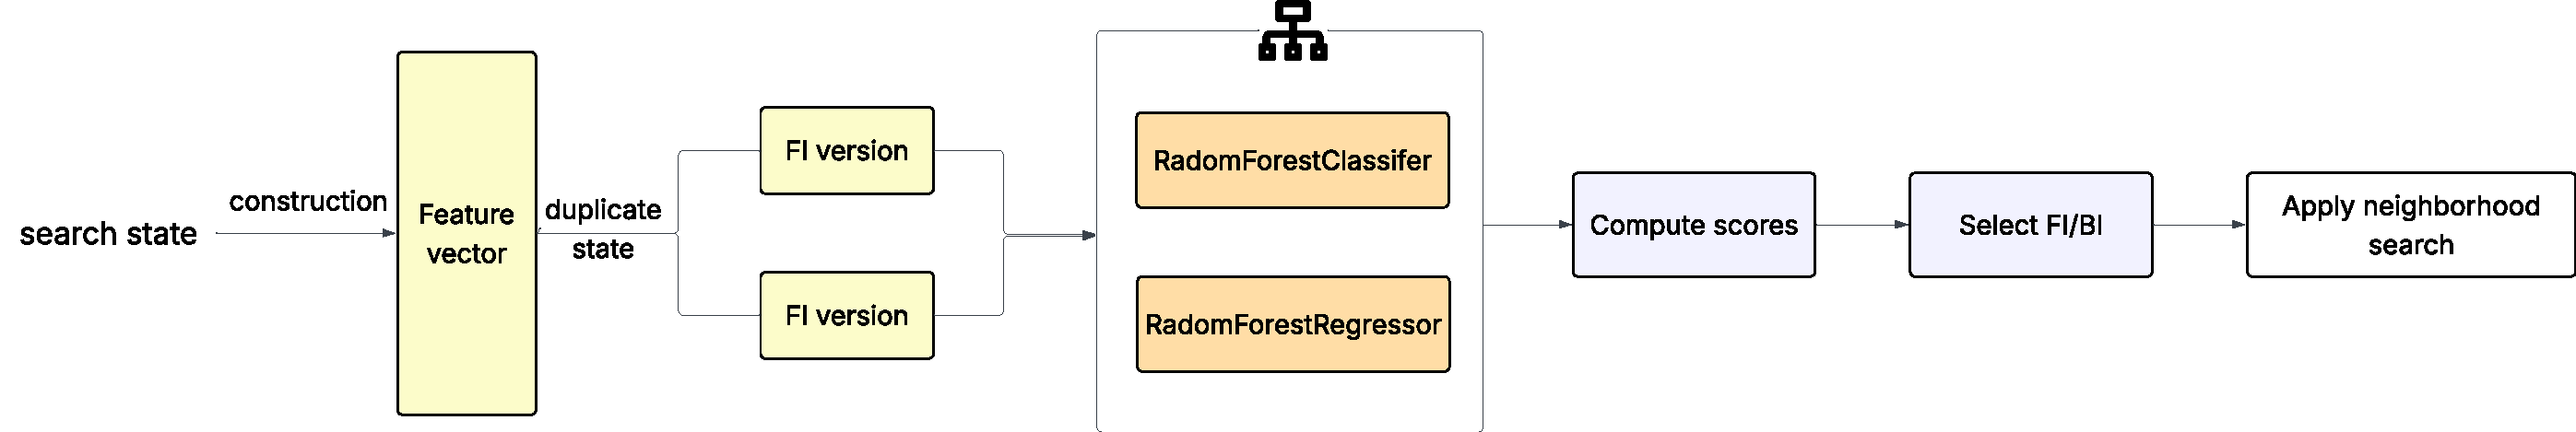
\includegraphics[width=\linewidth]
{../figures/rf_inference.pdf}

\caption{RF inference procedure}
\label{fig:rf_inference}
\end{figure}

%% ========= Integration into GVNS+ =========
\subsubsection{Integration into GVNS+}
The trained RF models are loaded once at the beginning of each optimization run. Before exploring a neighborhood during the B-VND procedure, the current search-state features are extracted and evaluated by the selector. The resulting decision determines whether the neighborhood is explored using FI or BI.

Algorithm~\ref{alg:rf_selector} summarizes the complete integration procedure.

\begin{algorithm}[ht]
\caption{RF-Based Adaptive Strategy Selection}
\label{alg:rf_selector}
\begin{algorithmic}[1]

\Require Current solution $S$, neighborhood $N_k$
\Ensure Candidate solution $S'$

\State Extract search-state features $\mathbf{x}$

\State Construct
$\mathbf{x}_{FI}=[\mathbf{x},0]$

\State Construct
$\mathbf{x}_{BI}=[\mathbf{x},1]$

\State Predict
$P_{FI}$ and $G_{FI}$

\State Predict
$P_{BI}$ and $G_{BI}$

\State Compute
$S_{FI}=P_{FI}\max(G_{FI},0)$

\State Compute
$S_{BI}=P_{BI}\max(G_{BI},0)$

\If{$S_{BI} > S_{FI}$}
    \State Apply neighborhood $N_k$ using BI
\Else
    \State Apply neighborhood $N_k$ using FI
\EndIf

\State Return resulting solution

\end{algorithmic}
\end{algorithm}

The proposed mechanism introduces an adaptive intensification layer within GVNS+, allowing the local-search strategy to evolve according to the current optimization context rather than remaining fixed throughout the search process.
